\section{Crane head}
On the head of the crane an Arduino Nano, an electromagnet, and an MPU-6050 gyroscope and accelerometer is mounted. The angle of the head is found by the Arduino Nano using data from the MPU-6050 as described in section \ref{sec:angleSensor}.  
The Arduino Nano transmits the angle using the outgoing serial interface which is connected to the TX-head of the DB-25 connector and the \textit{ANGLE}-output of the front panel. The baud-rate of the serial interface is \SI{9600}{\baud\per\second}. The data is sent in a decimal representation ending in a newline-character. 
%data from the MPU-6050 is sent on the Angle connection described in \ref{connector} using serial data with a baud-rate of 9600 and sending a decimal number formatted as a string ending with a new line character. 
%The electromagnet can be activated by sending a M1 command on the RX-head connection described in \ref{connector} and deactivated by sending M0 with a baud-rate of 9600 ending with a new line character. The connection to the head can be seen on figure \ref{fig:head}.
The electromagnet can be activated by sending "M1" and deactivated by sending an "M0" terminated by a new line character on the Rx-head connection with a baud rate of 9600. The connections to the head are shown in figure \ref{fig:head}.

\begin{figure}[H]
    \centering
    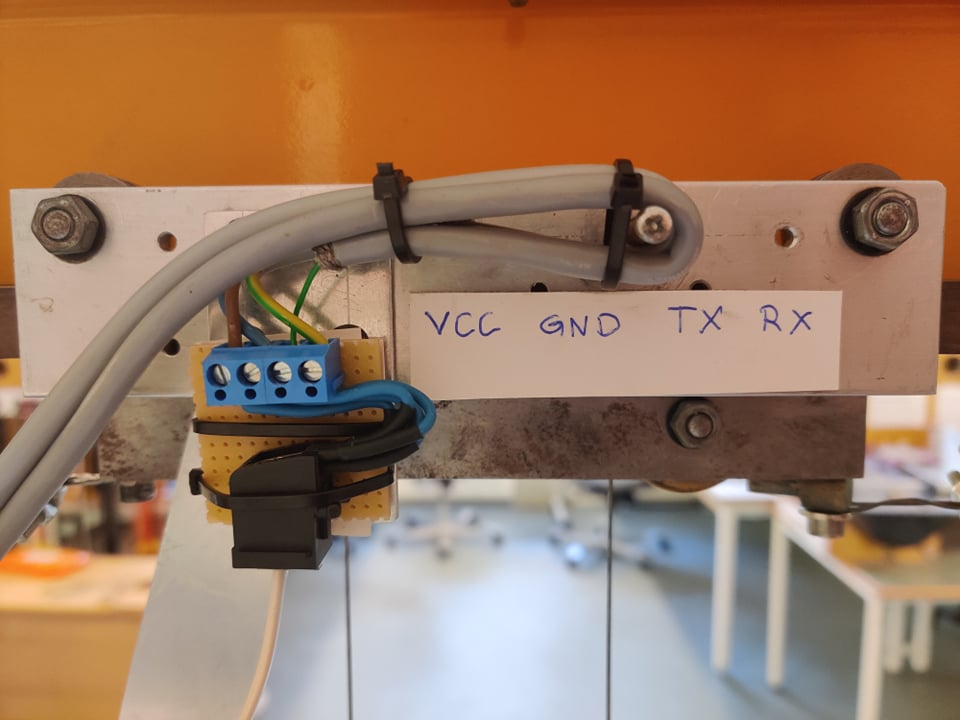
\includegraphics[width=0.6\textwidth]{pictures/head.jpg}
    \caption{Connections to head.}
    \label{fig:head}
\end{figure}

\subsection{Angle sensor}\label{sec:angleSensor}

%Since the crane head hangs from the trolley in compliant wires, it is essentially a pendulum. This means that movement of the x- and y-axis motors, will not exactly correspond to a similar movement of the crane head, since the pendulum will cause oscillations.

%In order to control these oscillations, it is necessary to know the angle of the head in relation to the surroundings at any given time. This should be done without disturbing the motion, which means that the sensor should be non-contacting between the crane and the swinging head. It is decided to accomplish this using an inertial measurement unit, attached to the crane head.

A small sensor and processor solution has been developed to measure the angle of the crane head, consisting of an Arduino Nano microprocessor and an MPU-6050 inertial measurement unit. The MPU consists of a 3-axis gyroscope and 3-axis accelerometer. Using a library for the MPU-6050, it is possible to utilize a built-in digital motion processor (DMP) to fuse the sensor inputs to estimate a set of pitch, roll and yaw angles. Since the head of the crane only swings in a single plane, using just the roll angle gives the desired result. The Arduino Nano sends the angle through a serial connection at \SI{9600}{\baud\per\second} as a decimal number encoded as a string of characters ending with a newline character to signal end of packet. Even though this means that mores bytes are needed to transmit the same information compared to simply transmitting the floating point variable, it does make decoding and troubleshooting easier.

A test is conducted in order to validate the accuracy and characteristics of the angle measurement. The test showed that the measured angle is within \SI{3}{\degree} of the actual angle measured using a video analysis tool named Tracker. The time delay of the sensor was measured to be \SI{38}{ms}.

\begin{figure}[H]
    \centering
    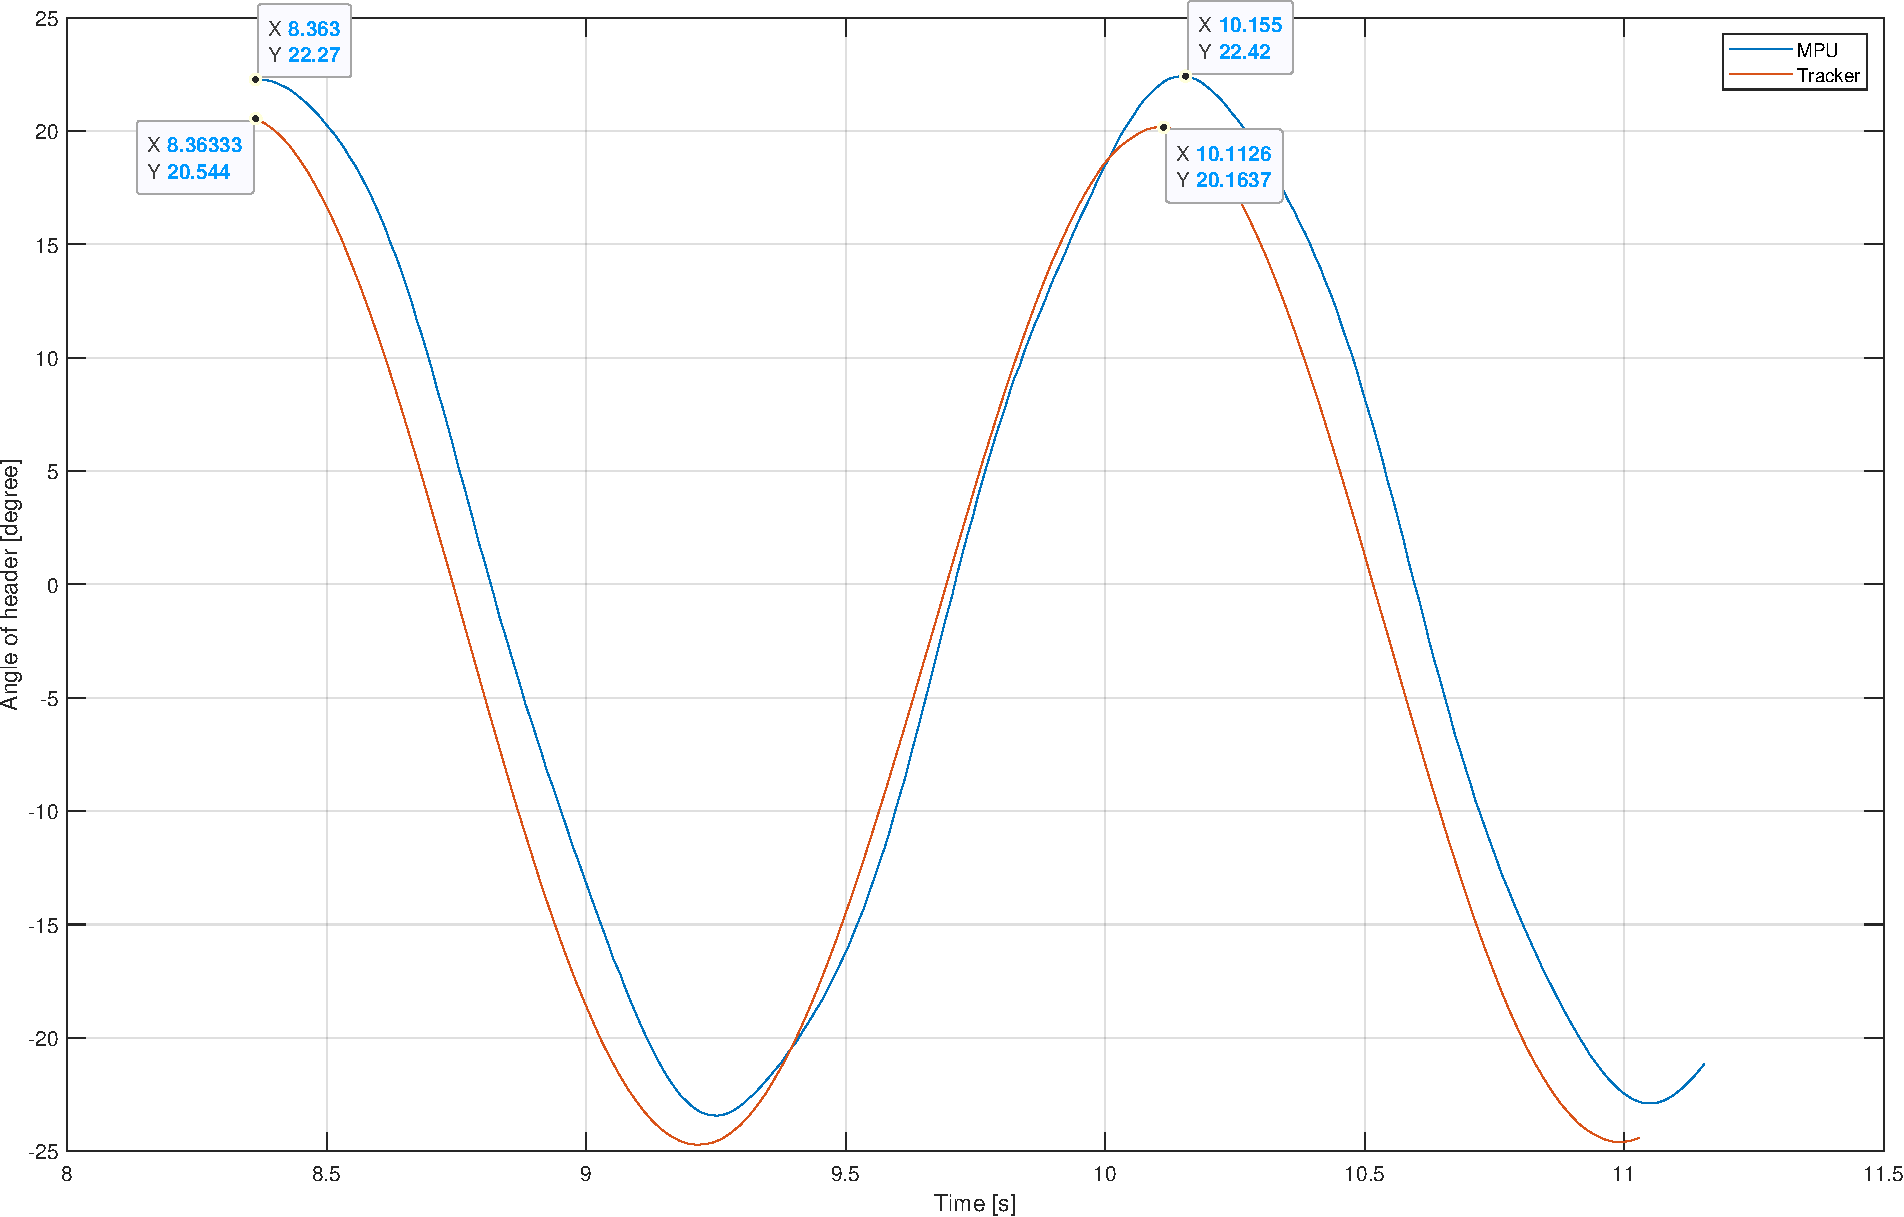
\includegraphics[width=0.7\textwidth]{pictures/angle_of_header.pdf}
    \caption{Meaured angle of head by the MPU compare to angle from Physlet Tracker. }
    \label{fig:res_angle_of_header}
\end{figure}


\textbf{links}

MPU6050:
\url{https://components101.com/sensors/mpu6050-module}

MPU6050 signal processing library:
\url{https://github.com/electroniccats/mpu6050}